\documentclass[a4paper]{IEEEtran}

% Packages
\usepackage{siunitx}
\usepackage{tikz}
\usepackage{graphicx}
\usepackage{url}

% NMEA spec environment
\newenvironment{nmeaspec}[1]
{
\newcommand{\field}[2]{\texttt{##1} & ##2 \\}
\vspace{0.2cm}
\noindent\texttt{#1}
\vspace{0.2cm}

\noindent Where: \vspace{0.1cm}\\  \noindent
\vspace{0.2cm}
\begin{tabular}{ll}
}
{
\end{tabular}
}

% Title, author, etc.
\title{\vspace{5.0cm}Autonomous surf life saving device}
\author{\Large Jarod Lam\\ \textit{Supervisor: Matthew Dunbabin}}
\IEEEspecialpapernotice{2018-2019 VRES project at Queensland University of Technology}

\begin{document}

% Title page
\begin{minipage}{\textwidth}
\vfill
\maketitle
\vfill
\end{minipage}
\clearpage

\tableofcontents

\begin{abstract}
build boat that saves people
\end{abstract}

\section{Introduction}
Surf life savers regularly patrol popular beaches to help those in danger, but there is a limit to the speed and ability of a human swimmer.

To supplement the activities of surf life savers at public beaches, a system has been proposed that will allow timely help to be given to people in danger while they wait to be rescued. The surf rescue boat (SRB) aims to deliver help quickly and reduce the risk to which life savers are exposed.

A simple water-based robot such as the one proposed can be constructed relatively cheaply and easily with off-the-shelf components. In the future, systems such as these may become widely available and save the lives of many along our coastal beaches. A prototype of one such robot was designed and built over the course of this project.

The system is divided into three main sections: a remotely operated water vehicle (the "boat"), an XBee-based radio communications system and protocol, and shoreline control. Out of these, only the vehicle and communications were prototyped in this project; the control system has been developed separately in the past and time constraints prevented it from being implemented.

This report describes these systems in detail, the design methodology, and avenues that can be explored for future development of the surf rescue boat.

\section{Boat}


% Todo: system overview figure

\subsection{Mechanical}
The remotely operated boat uses a standard surfboard as a base, and houses electronics in a watertight hard plastic case attached to the top. Two propellers are mounted to the bottom of the surfboard for movement control.

\subsubsection{Chassis}
Surfboard. Chosen for its stability and familiarity in the surf. The standardness and availability of surfboards is an advantage to encouraging development of such systems. A custom-built chassis may have been designed, but would have taken more time and money. 

\subsubsection{Propellors}
2 Blue Robotics T100 Thrusters. A propeller is mounted each to the left and right of the surfboard's middle underside. Aluminium mounting plates, attached to the board with Sikaflex, were designed to distribute force and allow propellors to be detached easily.

\subsubsection{Electronics housing}
Pelican 1120 Case. A laser-cut acrylic frame was made to mount the electronics in the box. Wire glands on the side of the box allow propellor wires to be fed through the box walls.

\subsection{Electronics}
An Arduino Mega 2560 controls the onboard electronics mounted in the case. GPS and IMU modules are used for navigation, and an XBee radio communicates with the base station. A block connection diagram of the electronics is shown in Figure \ref{elecdiag}.

\begin{figure}
\center
\pgfdeclarelayer{bg}
\pgfsetlayers{bg,main}
\begin{tikzpicture}

% Arduino
\draw [fill=teal!50] (0,0) rectangle ++(3,3) node [pos=0.5, align=center] (A) {Arduino Mega};

% Batteries
\draw [fill=blue!50] (A)++(-2.5,4.5) rectangle ++(1,-2) node [pos=0.5, rotate=90] (B1) {Battery 1};
\draw [fill=blue!50] (A)++(-1,4.5) rectangle ++(1,-2) node [pos=0.5, rotate=90] (B2) {Battery 2};

% ESCs
\draw [fill=yellow!50] (A)++(-3.5,-4.5) rectangle ++(0.5,2) node [pos=0.5, rotate=90] (E1) {ESC 1};
\draw [fill=yellow!50] (A)++(-2.5,-4.5) rectangle ++(0.5,2) node [pos=0.5, rotate=90] (E2) {ESC 2};

% XBee
\draw [fill=red!50] (A)++(1,4.5) rectangle ++(2,-2) node [pos=0.5] (X) {XBee};

% GPS
\draw [fill=green!80!black!20!white] (A)++(-1.5,-4.5) rectangle ++(2,2) node [pos=0.5] (G) {GPS};

% IMU
\draw [fill=red!50] (A)++(1,-4.5) rectangle ++(2,2) node [pos=0.5] (I) {IMU};

\begin{pgfonlayer}{bg}

% Power lines
\draw [red, thick] (E2)++(0.25,1) -- (B1) node [pos=0.5, rotate=90, above] {11.1V};
\draw [red, thick] (E1)++(0.25,1) -- ++(0,1.25) -- ++(1,0);
\draw [red, thick] (B2) -- ++(0,-1.5) -- ++(-1.5,0);
\draw [red, thick] (A) -- ++(-2,0);

% UART lines
\draw [blue, thick] (G) -- ++(0,2.75) node [pos=0.5, rotate=90, below] {UART};
\draw [blue, thick] (I) -- ++(0,1.5) -- ++(-1.5,0) node [pos=0.5, above] {UART} -- ++(0,1);
\draw [blue, thick] (X) -- ++(0,-1.5) -- ++(-1.5,0) node [pos=0.5, above] {UART} -- ++(0,-1);

% PWM lines
\draw [black, thick] (E2)++(-0.25,1) -- ++(0,0.3) -- ++(1.5,0) -- ++(0,1);
\draw [black, thick] (E1)++(-0.25,1) -- ++(0,0.5) -- ++(2.25,0) node[pos=0.45, above] {PWM} -- ++(0,1);

\end{pgfonlayer}

\end{tikzpicture}

\caption{Connection block diagram for onboard electronics.}
\label{elecdiag}
\end{figure}

\begin{figure}
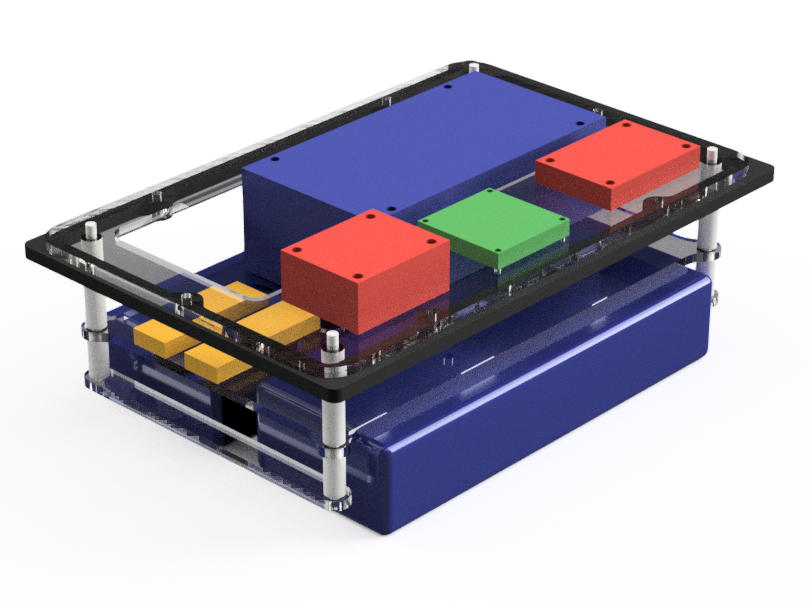
\includegraphics[width=\columnwidth]{assembly.png}
\caption{Rendering of internal electronics frame}
\label{elecframe}
\end{figure}

\subsubsection{Microcontroller}
Arduino Mega 2560 with Seeedstudio Grove Mega Shield breakout board. This development board is powerful enough to handle relatively simple communication and processing tasks required to control the boat's sensors and motors. More powerful ARM-based boards such as the Raspberry Pi are less suited to rugged environments, and more difficult to recover from failures. The shield provides robust headers to the UART functions of the Arduino.

\subsubsection{Radio}
Digi XBee Pro S1 on a SparkFun XBee Explorer Regulated. This connects to the Arduino via UART, and creates a wireless serial connection to the base station. The protocol is defined in section 3.

\subsubsection{GPS}
LOCOSYS LS20031 GPS receiver. Sends data to the Arduino via UART using the NMEA 0183 protocol found in section 3. 

\subsubsection{Orientation}
Sparkfun SEN-10736 9DOF Razor IMU. Sends data to the Arduino via UART. Currently, only the compass value from the sensor is used. Flashed with the Razor AHRS firmware: \url{https://github.com/Razor-AHRS/razor-9dof-ahrs}

\subsubsection{Motor control}
2 Flycolor Raptor 390 30A ESC. Firmware modified to allow forward and backward propeller movement. Receives PWM control signals from the Arduino with a duty cycle range of \SIrange{1000}{2000}{\micro\second}.

\subsubsection{Battery}
2 Zippy Flightmax Z58003S-30 \SI{5800}{mAh} 3S1P. The two batteries are wired in parallel, with a combined nominal capacity of \SI{11.6}{Ah} and nominal voltage of \SI{11.1}{V}.

\subsection{Software}
The Arduino Mega 2560 is programmed in C++ on top of Arduino default and custom libraries. Efforts were made to keep the code somewhat portable and reusable.

The code is split up into several modules, each handling a section of robot operation. These are described below, and the full code can be found in appendix A.

\subsubsection{\texttt{srb}}
Contains the main loop of the program. Initialises values, classes, etc. Runs update functions for GPS, comms, IMU, nav, and motors. Sends \texttt{SRBSM} message at intervals. An AVR watchdog timer is set to reset the microcontroller at the hardware level if the program hangs and reaches a timeout. 

\subsubsection{\texttt{nmea}}
Defines the \texttt{Nmea} class, which contains functions for constructing and parsing NMEA 0183 sentences. This includes generating and validating checksums, counting the number of fields, appending strings and decimal numbers to a sentence, and parsing a sentence by field. All functions use standard C string libraries, so they do not rely on Arduino libraries and will work outside the Arduino environment. Used by \texttt{SrbGps} and \texttt{SrbComms}.

\subsubsection{\texttt{srb\_stats}}
Defines the \texttt{SrbStats} class, which stores the ID, state, GPS and target location, compass and target heading, and other information related to the current state and navigation of the boat. A pointer to the same instance of this class is passed to most other classes when they are created so that they can read and update this information.

\subsubsection{\texttt{srb\_serial}}
Defines the \texttt{SrbSerial} class, which buffers a hardware serial stream and parses the input when a newline is received. The serial port used is configured when the object is created. This is the base class for \texttt{SrbGps}, \texttt{SrbComms}, and \texttt{SrbImu}.

\subsubsection{\texttt{srb\_gps}}
Defines the \texttt{SrbGps} class, which receives and parses GPS fix data over serial. Latitude, longitude, magnetic variation, and ground speed are parsed from the NMEA \texttt{GPRMC} sentence and stored in the \texttt{SrbStats} object. Conversions are made from knots to metres per second, and degrees/minutes to decimal degrees.

\subsubsection{\texttt{srb\_comms}}
Defines the \texttt{SrbComms} class, which sends and receives messages to and from the base station via the XBee radio. Contains functions for constructing and parsing the proprietary NMEA sentences defined in section 3. Stores information and instructions received in the \texttt{SrbStats} object. Stops the boat if no message is received within a timeout period.

\subsubsection{\texttt{srb\_imu}}
Defines the \texttt{SrbImu} class, which receives data from the Sparkfun IMU over serial. Extracts the compass heading from the serial stream and stores it in the \texttt{SrbStats} object.

\subsubsection{\texttt{srb\_motor}}
Defines the \texttt{SrbMotor} class, which controls motor movement. Receives motor power ranges from -100 to 100 and sets the corresponding PWM duty cycle. Accelerates motors to the desired speed at a safe pace.

\subsubsection{\texttt{srb\_nav}}
Defines the \texttt{SrbNav} class, which controls robot navigation. In manual mode, sets motor speed and orients the boat according to target speed and heading sent from the base station. In auto mode, moves the boat toward a set of coordinates sent from the base station. Motors are controlled with the \texttt{SrbMotor} class.

\section{Communications}
Communications between the SRB and the base station are done using XBee radios. By attaching a pair of XBee modules to the base station computer and the on-board Arduino, a virtual serial connection is effectively created between the two devices.

\subsection{NMEA 0183 protocol}
NMEA 0183 is a communications specification designed to create a standardised serial interface for GPS devices. Every NMEA `sentence' begins with a \texttt{\$} and ends with \texttt{*CS\textbackslash r\textbackslash n}, where \texttt{CS} is a two-digit hexadecimal checksum of the sentence.

A common NMEA sentence type is \texttt{GPRMC}, the GPS recommended minimum. \texttt{GPRMC} sentences are specified as follows: \cite{gpsinfo}

\begin{nmeaspec}{\$GPRMC,<Time>,<Status>,<Lat>,<LatDir>,\\<Lon>,<LonDir>,<Speed>,<Angle>,<Date>,\\<MagVar>,<MagDir>*CS}
\field{<Time>}{UTC timestamp in HHmmss format}
\field{<Status>}{Status \texttt{A}=active, \texttt{V}=void}
\field{<Lat>}{Latitude in ddmm.mmm format}
\field{<LatDir>}{\texttt{N} or \texttt{S} hemisphere}
\field{<Lon>}{Longitude in dddmm.mmm format}
\field{<LonDir>}{\texttt{E} or \texttt{W} hemisphere}
\field{<Speed>}{Ground speed in knots}
\field{<Angle>}{Track angle in degrees from north}
\field{<Date>}{Date in DDMMYY format}
\field{<MagVar>}{Magnetic variation magnitude}
\field{<MagDir>}{Magnetic variation direction}
\end{nmeaspec}

A NMEA sentence parser was written for the SRB to interpret messages from the on-board GPS and extract location information.

\subsection{Proprietary NMEA sentences}
Some advantages of using NMEA sentences are that they are standardised, human-readable, robust, and relatively simple to implement. Specified below is a set of custom NMEA sentence types was created for communication between the boat and the base station.

\subsubsection{SRBSM - Status Message}
The \texttt{SRBSM} sentence is sent periodically by the boat to update the base station with status information.

\begin{nmeaspec}{\$SRBSM,<ID>,<State>,<Lat>,<Lon>,<Speed>,\\<Heading>,<BattV>,<FwdPower>,\\<TgtHeading>*CS}
\field{<ID>}{ID of target SRB}
\field{<State>}{\texttt{0}=disabled, \texttt{1}=manual, \texttt{2}=auto}
\field{<Lat>}{Latitude in decimal degrees}
\field{<Lon>}{Longitude in decimal degrees}
\field{<Speed>}{Speed in metres per second}
\field{<Heading>}{Compass heading in degrees CW from north}
\field{<BattV>}{Current battery voltage}
\field{<FwdPower>}{Forward power from -100 to 100}
\field{<TgtLat>}{Target latitude in decimal degrees}
\field{<TgtLon>}{Target longitude in decimal degrees}
\field{<TgtHeading>}{Target heading in degrees CW from north}
\end{nmeaspec}

\subsubsection{SRBJS - Joystick}
The \texttt{SRBJS} sentence is sent by the base station for manual control of the boat.

\begin{nmeaspec}{\$SRBJS,<ID>,<FwdPower>,<TgtHeading>*CS}
\field{<ID>}{ID of target SRB}
\field{<FwdPower>}{Forward power from -100 to 100}
\field{<TgtHeading>}{Target heading in degrees CW from north}
\end{nmeaspec}

\subsubsection{SRBWP - Waypoint}
The \texttt{SRBWP} sentence is sent by the base station to autonomously direct the boat to a set of coordinates.

\begin{nmeaspec}{\$SRBJS,<ID>,<TgtLat>,<TgtLon>*CS}
\field{<ID>}{ID of target SRB}
\field{<TgtLat>}{Target latitude in decimal degrees}
\field{<TgtLon>}{Target longitude in decimal degrees}
\end{nmeaspec}

\section{Testing}

\section{Future development}

\bibliography{bibliography}
\bibliographystyle{IEEEtran}

\clearpage
\onecolumn
\appendices

\section{Code}
\subsection{the codes}

\section{Drawings}
\subsection{the drawings}

\end{document}